\chapter{Astrophysical Radiation}
\label{chapter:astro_rad}

As discussed in Chapter~\ref{chapter:eor_intro}, the target signal of EoR experiments has a brightness temperature of order $\sim 10$\,mK. At the $50-200$\,MHz frequencies for these experiments, however, foreground radiation from the Milky Way (referred to as `the Galaxy', with a capital `G' for much of this thesis), extragalactic sources and manmade interference, with total brightness temperature $\sim 10^4$ times greater than the target signal, is the principle challenge to overcome \citep[e.g.][]{Santos.05, GSM.08, Bernardi.09, Bernardi.10, Pober.13, Dillon.14, Kohn.16, Kohn.18}. In this Chapter, I outline our current understanding of polarized and unpolarized foregrounds, and the implications for the dynamic range required for an EoR detection. The Southern Hemisphere is the focus of the chapter, as this is where the instruments used in this work are based (see Chapter~\ref{chapter:instruments}). For a comprehensive review of radiative processes in astrophysics, see \cite{Rybicki.79}. 

\section{Synchrotron Radiation}

Any accelerating charged particle will radiate. For low-frequency radio foregrounds, the radiation we are most interested in is emitted by electrons accelerated by Galactic magnetic fields.
At non-relativistic velocities, the radiation of a charged particle accelerated by magnetic field $\vec{B}$ is well-described by relatively simple formulae, and is referred to as `cyclotron radiation'. In this case, the emission spectrum is simply determined by gyration frequency about the magnetic field lines.
At relativistic velocities, the spectrum becomes more complicated, and is referred to as `synchrotron radiation'.

The equation of motion of a relativistic charged particle of mass $m$, charge $q$ and velocity $\vec{v}$ can be written as 
\begin{equation}
\frac{{\rm d}}{{\rm d}t}(\gamma m \vec{v}) = \frac{q}{c}\vec{v}\times\vec{B},
\label{eq:astropol_eom_b}
\end{equation}
where $\gamma$ is the Lorentz factor, and
\begin{equation}
\frac{{\rm d}}{{\rm d}t}(\gamma m c^2) =q \vec{v}\cdot\vec{E} = 0,
\label{eq:astropol_eom_e}
\end{equation}
where $\vec{E}$ is the electric field. Equation~\ref{eq:astropol_eom_e} implies that either $\gamma$ or $|\vec{v}|=v$ are constant. Therefore, we may write
\begin{equation}
\gamma m\frac{{\rm d}\vec{v}}{{\rm d}t} = \frac{q}{c}\vec{v}\times\vec{B}.
\end{equation}
Decomposing the velocity into components perpendicular and parallel to $\vec{B}$,
\begin{equation}
\frac{{\rm d}\vec{v}_{\parallel}}{{\rm d}t} = 0;\,\,\,\,\,\frac{{\rm d}\vec{v}_{\perp}}{{\rm d}t} = \frac{q}{\gamma m c} \vec{v}_{\perp}\times\vec{B},
\end{equation}
we find that $\vec{v}_{\parallel}$ is constant, and as $v$ is constant, so $\vec{v}_{\perp}$ must be also. This proves that motion along the magnetic field lines is helical, with gyration frequency
\begin{equation}
\omega_B = \frac{qB}{\gamma m c}.
\end{equation}
Using the covariant form of the Larmor Formula with the magnitude of acceleration perpendicular to the magnetic field $a_{\perp} = \omega_B v_{\perp}$, the total emitted radiation has power
\begin{equation}
P = \frac{2 q^2}{3c^3}\gamma^4 a_{\perp}^2,
\end{equation}
which when accounting for an isotropic velocity distribution, reduces to
\begin{equation}
P = \frac{4}{24\pi}\sigma_T c \beta^2 \gamma^2 B^2
\end{equation}

Since the electrons follow a helical path, an observer will only see components of the emission when the motion is parallel to the line-of-sight. The observed radiation will be emitted along path $\delta s$ with radius of curvature $r$ and and angle $\delta \theta$, such that $\delta\theta = 2/\gamma$ and $\delta s = 2r/\gamma$. Equations~\ref{eq:astropol_eom_b} and \ref{eq:astropol_eom_e} grant
\begin{equation}
r = \frac{v}{\gamma\omega_B\sin\alpha},
\end{equation}
where $\alpha$ is the angle between $\vec{v}$ and $\vec{B}$. The time taken for the electron to travel $\delta s$, and therefore emit the observed radiation, may be characterized by a critical frequency
\begin{equation}
\omega_c = \frac{3}{2}\gamma^3\omega_B\sin\alpha.
\end{equation}

Deferring to \cite{Rybicki.79} for a full discussion, the frequency spectrum of synchrotron radiation is intimately tied to the helical geometry of the problem and $\omega_c$, with power per unit frequency proportional to some function $F(\omega/\omega_c)$:
\begin{equation}
P(\nu) = \frac{\sqrt{3}q^3B\sin\alpha}{m_e c^2}F(\frac{\omega}{\omega_c})
\label{eq:astropol_sync_power}
\end{equation}
where the form of $F$ depends on the energy distribution of the electrons. For black-body radiators in the Rayleigh-Jeans limit, appropriate for low-frequency radio observations, the number density of particles with energy $E$ can be described with a power law:
\begin{equation}
N(E){\rm d}E = AE^{-p}{\rm d}\gamma ,
\end{equation}
where $A$ is a constant of proportionality that can vary with angle of observation. In this case, it can be shown that the total energy density per unit frequency is
\begin{equation}
P(\nu) = \frac{A\sqrt{3}q^3B\sin\alpha}{m_e c^2 (p+1)}\left(\frac{2\pi mc}{3qB\sin\alpha}\nu\right)^{-{\frac{p-1}{2}}}\Gamma\left(\frac{p}{4} + \frac{19}{12}\right)\Gamma\left(\frac{p}{4} - \frac{1}{12}\right).
\end{equation}

The objective of this exercise was to show that the total power of synchrotron radiation is innately smooth as a function of frequency; it can be described as a power law. An example observation of low-frequency Galactic synchrotron is shown in Figure~\ref{fig:astropol_edges_spec}. The observed sky spectrum has a spectral index $\beta_*=2.52\pm0.04$ for brightness temperature $T(\nu)\propto\nu^{-\beta_*}$. Recall that the {\sc hi} EoR field has a complex structure in both the image plane and along the line-of-sight (c.f. Figure~\ref{fig:eor_intro_plp_sim}). The superposition of emission lines from this field will lead to unsmooth, structured emission per unit frequency.
In the face of synchrotron foregrounds being many orders of magnitude brighter than the 21\,cm emission, \textit{this difference in spectral behavior is the single most important distinguishing feature between foregrounds and the EoR}.

\begin{figure}
\centering
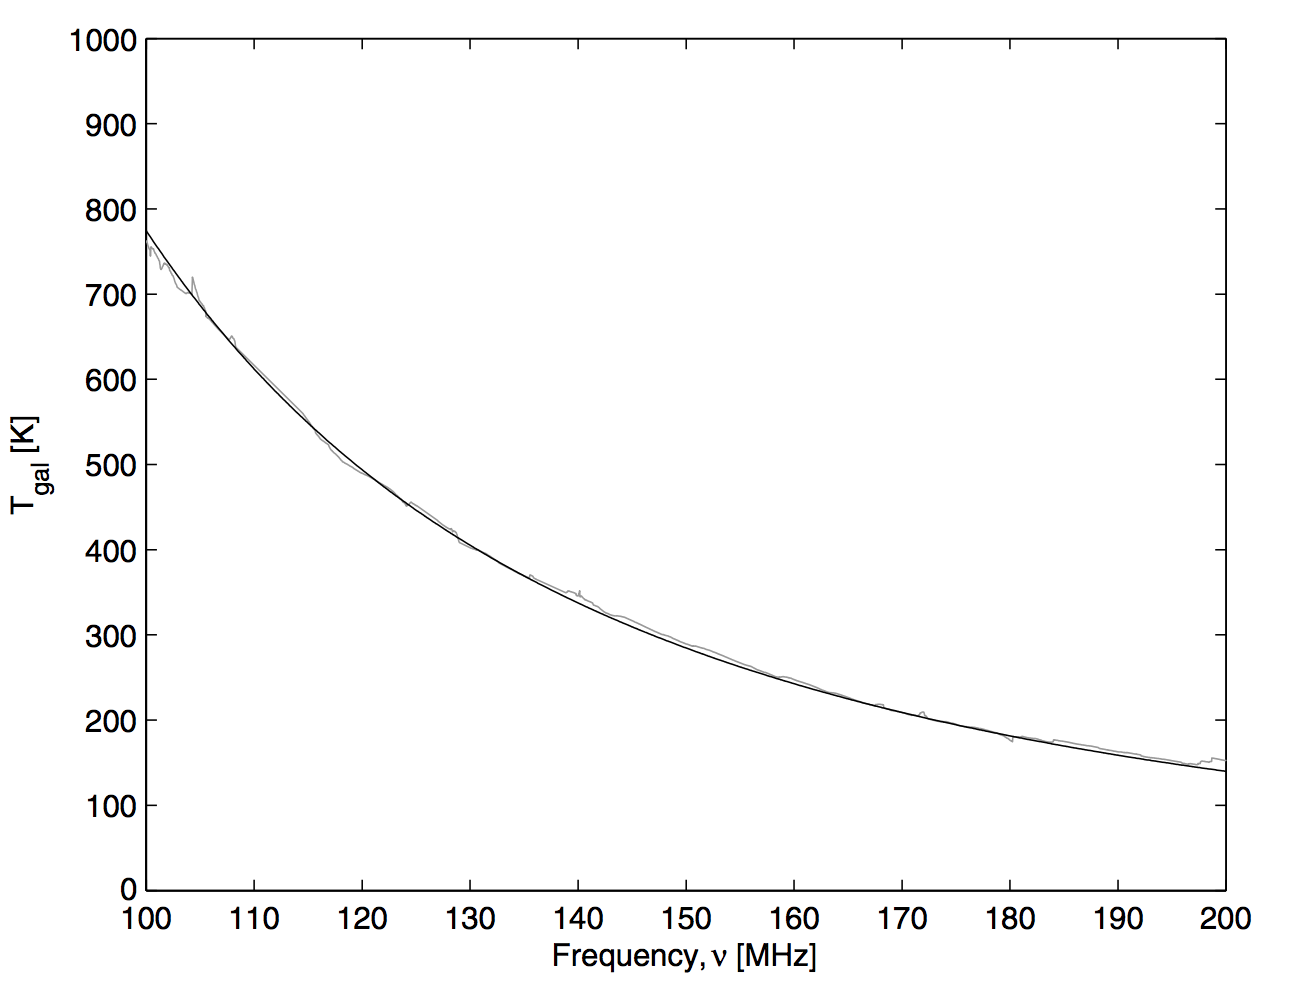
\includegraphics[width=0.75\textwidth]{chapters/astropol/figures/edges_spectrum.png}
\caption[The low-frequency synchrotron spectrum of the sky, as measured by \cite{Rogers.08}.]{The low-frequency synchrotron spectrum of sky, measured by \cite{Rogers.08}. Their measurement is shown in light grey, overlaid with a well-fit power law of spectral index $2.52\pm0.04$.}
\label{fig:astropol_edges_spec}
\end{figure}

\section{Stokes parameters}

It is extremely unlikely that we will observe radiation from electrons spiralling along magnetic field lines that are exactly parallel or perpendicular to our line-of-sight. Instead, some elliptically polarized component of the radiation is observed. The Stokes parameters are quantities used to describe the polarization state of electromagnetic waves.

We can describe a monochromatic electromagnetic wave propagating towards the observer as the real part of 
\begin{equation}
\vec{E} = \vec{E}_0e^{-i\omega t} = \begin{pmatrix}
E_1 e^{i\phi_1}\\
E_2 e^{i\phi_2}
\end{pmatrix}e^{-i\omega t}
\end{equation}
It can be shown \citep[e.g.][]{Rybicki.79} that the real part of the vector above can be mapped, in general, to the principle axes of an ellipse at position angles $\psi$ and $\chi$ to the Cartesian plane, as shown in Figure~\ref{fig:astropol_pol_ellipse}. These two angles, $E_1$, and $E_2$, can be used to define the Stokes parameters for monochromatic waves:
\begin{align}
I &\equiv E_1^2 + E_2^2 = E_0^2, \\
Q &\equiv E_1^2 - E_2^2 = E_0^2\cos 2\psi \cos 2\chi,\\
U &\equiv 2E_1E_2\cos(\phi_1 - \phi_2) = E_0^2\cos 2\chi \sin 2\psi, \\
V &\equiv 2E_1E_2\sin(\phi_1 - \phi_2) = E_0^2\sin 2\chi.
\end{align}

The interpretation of these parameters is as follows: Stokes I measures the total intensity of the electric field. Stokes Q and U measure the orientation of the electric field relative to, in this case, the $x$-axis of the Cartesian plane, where Q measures the projection parallel to the $x$-axis and U measures the projection at $45^{\circ}$ to the $x$-axis. They are clearly linked, as $\tan\psi = U/Q$. Stokes V is the circularity parameter, measuring the ratio of the principle axes of the ellipse. For monochromatic waves, $I^2 = Q^2 + U^2 + V^2$.

\begin{figure}
\centering
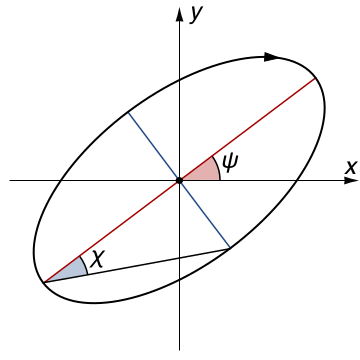
\includegraphics[width=0.5\textwidth]{chapters/astropol/figures/pol_ellipse.png}
\caption{A representation an elliptically polarized monochromatic wave with respect to the Cartesian grid.}
\label{fig:astropol_pol_ellipse}
\end{figure}

In practice, observed radiation fields are rarely monochromatic (purely elliptically polarized). Instead, we observe a superposition of electric fields, each with its own polarization state. If we assume that the amplitude and phase of the observed radiation change relatively slowly over time, we can express 

\begin{equation}
\vec{E}(t) = \vec{E}_0(t)e^{-i\Phi(t)} = \begin{pmatrix}
E_1(t) e^{i\phi_1(t)}\\
E_2(t) e^{i\phi_2(t)}
\end{pmatrix}
\end{equation}
such that over short times $\Delta t \sim 1/\omega$ the wave is of a definite elliptical polarization state, but for $\Delta t \gg 1/\omega$ the polarization state can change by a large amount. Such waves are referred to as `quasi-monochromatic', with coherence time $\Delta t$ and its conjugate, bandwidth $\Delta\omega$. Due to the time-dependent nature of quasi-monochromatic waves, the exact values of $E_1$, $E_2$, $\phi_1$ and $\phi_2$ cannot be precisely measured. Instead, radiometers measure the average sum of squares of the components of $\vec{E}(t)$. These can be used to define the Stokes parameters for quasi-monochromatic waves:

\begin{align}
I &\equiv  \left\langle E_1E_1^* \right\rangle + \left\langle E_2E_2^* \right\rangle = \left\langle E_1^2 + E_2^2 \right\rangle, \\
Q &\equiv \left\langle E_1E_1^* \right\rangle - \left\langle E_2E_2^* \right\rangle = \left\langle E_1^2 - E_2^2 \right\rangle, \\
U &\equiv \left\langle E_1E_2^* \right\rangle + \left\langle E_2E_1^* \right\rangle = \left\langle 2 E_1 E_2 \cos(\phi_1 - \phi_2)\right\rangle, \\
V &\equiv -i (\left\langle E_1E_2^* \right\rangle - \left\langle E_2E_1^* \right\rangle) = \left\langle 2 E_1 E_2 \sin(\phi_1 - \phi_2)\right\rangle, \\
\end{align}
where $E_i^*$ indicates the complex conjugate of $E_i$, and $\left\langle \cdots \right\rangle$ indicates an average over some integration time over which the measurement is made. It is easy to see from the Cauchy-Schwarz inequality that for quasi-monochromatic waves, $I^2 \geq Q^2 + U^2 + V^2$. Radiation is completely unpolarized if $Q=U=V=0$. It it common to refer to the `polarization fraction' or `degree of polarization' of observed radiation, $p$:

\begin{equation}
p \equiv \frac{\sqrt{Q^2 + U^2 + V^2}}{I}
\end{equation}
and `linear polarized intensity', $P$:

\begin{equation}
P = \frac{1}{2}\sqrt{Q^2 + U^2}
\end{equation}

The Institute of Electrical and Electronics Engineers (IEEE) defines the standard reference frame for the polarization axes to be the lines of constant Right Ascension ($\alpha$) and Declination ($\delta$) on the sky. Substitution of $1\rightarrow\alpha$ and $2\rightarrow\delta$ in the definitions above brings those definitions to standard \citep{Cohen.58, Ludwig.73, vanStraten.10}.

\section{Total intensity foregrounds}

At EoR frequencies, $50 - 250$\,MHz, the brightest source of total intensity is the Galactic Plane. While the configuration of the Galactic magnetic field is still a matter of debate \citep[e.g.][]{Haverkorn.15}, but observations of synchrotron emission suggest it has an average power of $\sim6\mu$G \citep[e.g.][]{Beck.03}. Multiple, dynamic sources of {\sc hii} such as supernova remnants (SNRs) and other contributors to the interstellar medium provide charged particles to radiate synchrotron. This has a brightness temperature of $\sim$5\,K. Beyond our Galaxy, synchrotron from extragalactic sources (galaxies and galaxy clusters) have brightness temperatures $\sim$0.5\,K \citep[e.g.][]{Jelic.10}. 

With the advent of newly operational low-frequency interferometers (see Chapter~\ref{chapter:instruments}), detailed maps of low-frequency synchrotron emission in the Southern Hemisphere have only very recently become accessible. 
The PAPER-64 imaging array \citep[][and Chapter~\ref{chapter:instruments}]{Jacobs.11, Jacobs.13, Stefan.13} was used to make a map of the Southern Galactic Plane at 145\,MHz. This array was able to resolve some diffuse components, but mainly focused on relatively small-scale structures such as SNRs and {\sc hii} regions (i.e. tens of parsecs; \citealt{Asvarov.14}). That map is shown in Figure~\ref{fig:astropol_galplane_paper}, projected into Galactic coordinates. Synchrotron sources in the plane of the Galaxy include SNRs (most prominently the Vela and Puppis complexes to the East), {\sc hii} regions (almost indistinguishable from SNRs in the plane) and ionized gas. Above and below the Galactic plane, extragalactic point sources are visible (and match the \cite{Jacobs.11} 145\,MHz point-source catalog of the region).

\begin{figure}
\centering
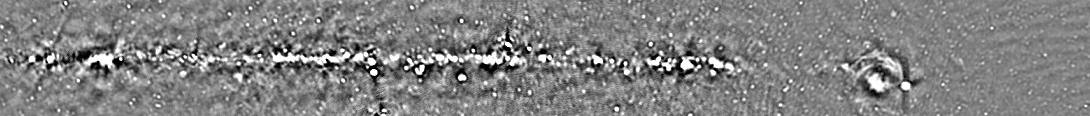
\includegraphics[width=0.9\textwidth]{chapters/astropol/figures/galplane_linscale.png}
\caption[The Southern Galactic Plane as observed by PAPER-64 at 145\,MHz.]{The Galactic plane as observed by PAPER-64. Synchrotron sources include supernova remnants (e.g. the Vela and Puppis complexes to the East), {\sc hii} regions and ionized gas in the plane of the Galaxy. Extragalactic sources are visible above and below the Galactic plane.}
\label{fig:astropol_galplane_paper}
\end{figure}
% GSM -- collection of data including very diffuse components
Motivated by the sparsity of wide-field, diffuse radio surveys, \cite{GSM.08} presented the `Global Sky Model' (GSM), in which they amalgamated as many high-fidelity wide-field radio surveys as possible, from 10\,MHz to 100\,GHz. \cite{GSM.17} extended the upper limit of this range to 10\,THz. Using principal component analysis and an expectation for smooth frequency structure, they were able to build a model that could be interpolated to any requested frequency within their spectral range. An example at 150\,MHz is shown in Figure~\ref{fig:astropol_gsm}. It is important to note that the GSM is uncertain at the $\sim$5\% level, and in the southern hemisphere this uncertainty is greater due to fewer well-characterized surveys of diffuse emission. Aside from diffuse Galactic emission, the GSM also includes the `A Team' of bright radio sources, such as Pictor A, Fornax A and Centaurus A. Pictor A is particularly useful as a calibration source: it is relatively unpolarized, unresolved as a point source, and the one of the brightest extragalactic sources of synchrotron emission \citep{Jacobs.13}.

\begin{figure}
\centering
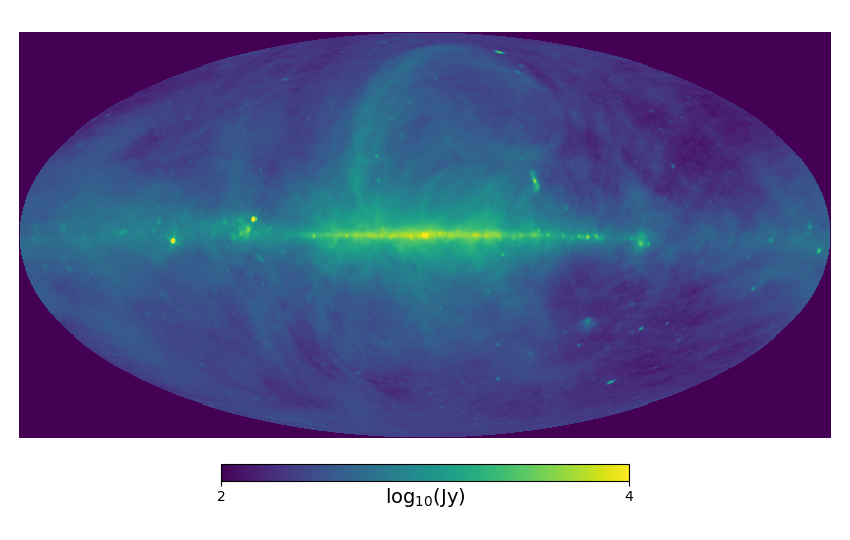
\includegraphics[width=0.75\textwidth]{chapters/astropol/figures/gsm.png}
\caption{The GSM at 150\,MHz: a relatively accurate model of diffuse synchrotron across the entire sky.}
\label{fig:astropol_gsm}
\end{figure}

With the advent of the 128-tile Murchinson Widefield Array (MWA), the GaLactic and Extragalactic All-sky Murchison Widefield Array (GLEAM) survey took place over two years, imaging most of the sky south of Declination $+25^{\circ}$ in Stokes I, Q, U \& V with myriad science goals \citep{Bowman.13, Wayth.15, Hurley-Walker.17}. Covering 70--230\,MHz with 10\,kHz frequency resolution, sensitivity to a wide range of spatial scales, and reaching theoretical noise levels in Stokes I, GLEAM (the maps of which are not yet public) will have a significant legacy for our understanding of the low-frequency sky. 

\section{Linearly Polarized Foregrounds}
\label{sec:astropol_linpol_fgs}
Polarized foregrounds are less well characterized than total intensity ones, especially in the southern hemisphere, and even then, the measurements were typically at GHz frequencies and must be extrapolated for relevance to EoR studies. The DRAO 26\,m \citep{Wolleben.06} telescope and the VLA \citep{Condon.98} mapped the entire sky, in Stokes I, Q, U \& V, visible from their respective positions in the northern hemisphere. This meant that much of the southern hemisphere was blocked by the Earth. Both of these surveys were performed at 1.4\,GHz. The polarized intensity map produced by \cite{Wolleben.06} is shown in Figure~\ref{fig:astropol_drao_map} in Galactic coordinates.

\begin{figure}
\centering
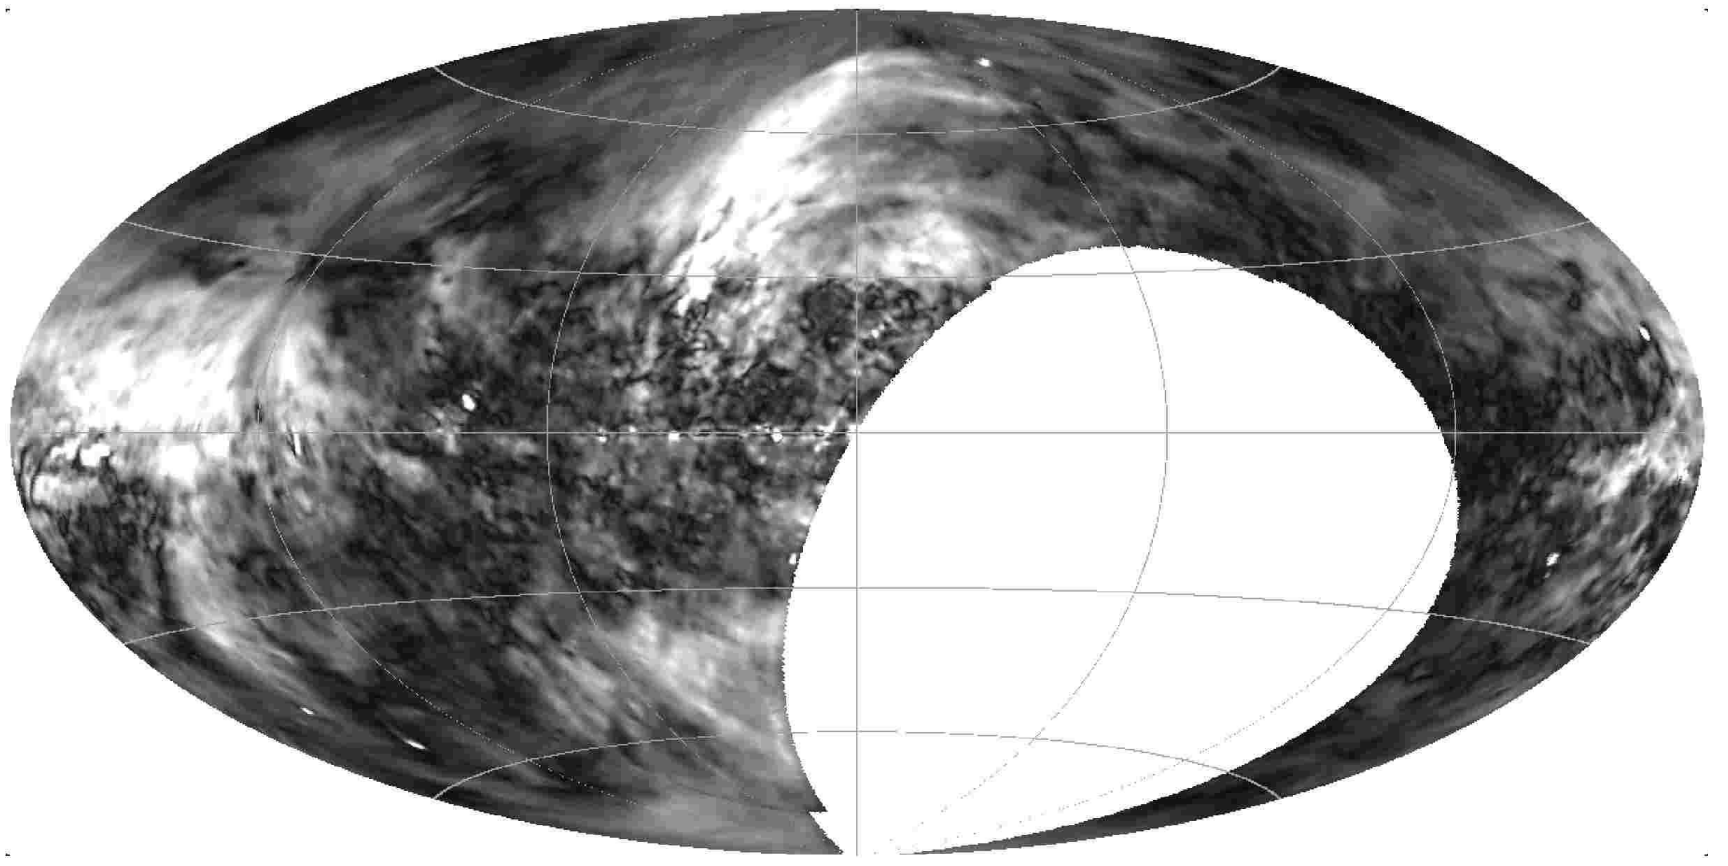
\includegraphics[width=0.7\textwidth]{chapters/astropol/figures/drao_map.png}
\caption{The polarized intensity of the sky as viewed by the DRAO 26\,m telescope at 1.4\,GHz. Figure taken from \cite{Wolleben.06}.}
\label{fig:astropol_drao_map}
\end{figure}

\cite{Bernardi.13} surveyed 2400\,deg$^2$ of the southern hemisphere with the 32-element MWA at 189\,MHz in Stokes I, Q and U. They detected large amounts of bright ($\sim 10$\,K), diffuse polarized emission at hour angles close to the transit of the Galaxy (most likely the contribution of diffuse emission south of the Galactic Plane, as visible in Figure~\ref{fig:astropol_drao_map}), but just one polarized extragalactic source with flux density $>4$\,Jy. 

Indeed, most recent observations in the 100--200 MHz band, covering selected sky areas, have revealed that bright Galactic diffuse polarized synchrotron radiation seems to be ubiquitous \citep{Bernardi.09, Bernardi.10, Jelic.14, Lenc.16} with peak emission up to 15 K \citep{Jelic.15}, but find a dearth of bright polarized (extragalactic) point sources. The point sources cataloged by \cite{Bernardi.13} showed significant depolarization compared to their polarized flux density at higher frequencies (see Section~\ref{subsec:astropol_depolar}). 

As calibration schemes are refined and modern interferometers grow, a small population of weakly polarized point sources has recently been revealed. Observing $\sim 625$\,deg$^2$ with the 128-element MWA, at 154\,MHz, \cite{Lenc.16} found five polarized point sources of polarized intensity order $10-100$\,mJy\,beam$^{-1}$. Much deeper integrations with the Low Frequency Array (LOFAR) presented by \cite{VanEck.18} found 92 polarized point sources within 570\,deg$^2$, observed at 150\,MHz, with polarized intensities of the  order $1-10$\,mJy\,beam$^{-1}$. In all of these observations, polarized intensity represented a polarized fraction $p\leq 15$\%.

Note that we have focused on polarized intensity -- Stokes Q and U -- for this discussion.
At low frequencies, Stokes V is expected to be almost intrinsically zero \citep[e.g.][]{Sokolowski.17}. While at higher frequencies circularly polarized synchrotron has been observed from sources such as relativistic jets \citep[e.g.][]{Macquart.04}, very few natural sources of Stokes V are present in the low frequency sky, with the exception of transients such as extrasolar flares \citep{Spreeuw.10} and aurorae of giant planets \citep[e.g.][]{Zarka.05, Badman.15}. This makes measurements of Stokes V useful for null tests \citep[e.g.][]{Patil.17}

\subsection{Faraday Rotation}

One of the most important considerations for {\sc hi} EoR measurements is the Faraday Rotation Measure of polarized foregrounds (the reasons for this are thoroughly enumerated in Chapter~\ref{chapter:eor_window_theory}). 

Electromagnetic waves will undergo dispersion and refraction while propagating through and ionized gas or plasma. If an external magnetic field is incident upon the plasma, electrons in the plasma will gyrate about the field with frequency
\begin{equation}
\omega_B = \frac{e}{m_e c}B_0 \approx 1.67\times 10^7 B_0 {\rm\, s^{-1}},
\end{equation}
where $B_0$ is the magnitude of the magnetic field. This alters the dielectric constant in the plasma.
Decomposing linearly polarized radiation in to a circular basis (this basis change is not the equivalent of intrinsically circularly polarized Stokes V radiation) of clockwise (`right-handed'; R) and anti-clockwise (`left-handed'; L) waves, we can express the dielectric constant as
\begin{equation}
\epsilon_{R,L} = 1 - \frac{\omega_P^2}{\omega(\omega \pm \omega_B)},
\end{equation}
where R and L correspond to + and -, respectively, $\omega$ is the angular frequency of the radiation, and $\omega_P$ is the plasma frequency
\begin{equation}
\omega_P^2 = \frac{4\pi n_e e^2}{m_e},
\end{equation}
for electron number density $n_e$. The index of refraction of a plasma is given by $\sqrt{\epsilon}$. Clearly, the handedness of the radiation will experience different angles refraction. The effect of this in the linear basis is to rotate the plane of polarization as the radiation propagates through the magnetized plasma. For a screen of width $L$, the change in angle is given by \citep{Rybicki.79, TMS}:
\begin{equation}
\Delta\phi = \frac{1}{2}\int^L_0 \frac{\omega_P^2\omega_B}{c\omega^2}{\rm d}l.
\end{equation}
Substituting for $\omega_B$ and $\omega_P$, and observing the radiation along the line-of-sight (as we must), gives
\begin{equation}
\Delta\phi = \frac{e^3}{(m_e c^2)^2}\lambda^2 \int^L_0 n_e(l)B_{\parallel}(l) {\rm d}l \equiv \lambda^2\Phi
\end{equation}
where we have moved from angular frequency to wavelength, and defined the \textit{Faraday Rotation Measure} (RM) $\Phi$. This rotation moves power between Stokes Q and U,
\begin{equation}
(Q + iU)_{\rm observed} = e^{-2i\Phi\lambda^2}(Q + iU)_{\rm intrinsic},
\label{eq:astropol_faraday_rotation}
\end{equation}
where $\Phi$ has units of rad\,m$^{-2}$.

At GHz radio frequencies, measurements of polarization angle with respect to wavelength can be used to chart the magnetic field of galaxies, given some independent measure of the electron number density. Equation~\ref{eq:astropol_faraday_rotation} also defines a Fourier relationship between $\Phi$ and $\lambda^2$, which can be exploited to obtain a similar measurement, and is referred to as `RM synthesis' \citep{Brentjens.05}. Importantly, at low frequencies the large values of $\lambda$ will cause rapid phase wraps for RMs $\geq \sim 10$, inducing spectral structure in what would otherwise be smooth synchrotron spectra \citep{Moore.13}. 

Figure~\ref{fig:astropol_rm_map} shows the all-sky RM measurements of \cite{Oppermann.12}, obtained by using both of the above methods (fitting in $\lambda^2$ and RM synthesis) on a number of radio surveys ranging from $1.1$ to $11$\,GHz. Uncertainties in the values reported are typically at the level of $\sim$10\%, with larger uncertainties in the southern hemisphere due to fewer polarization surveys existing in that region, and along the Galactic plane. 

\begin{figure}
\centering
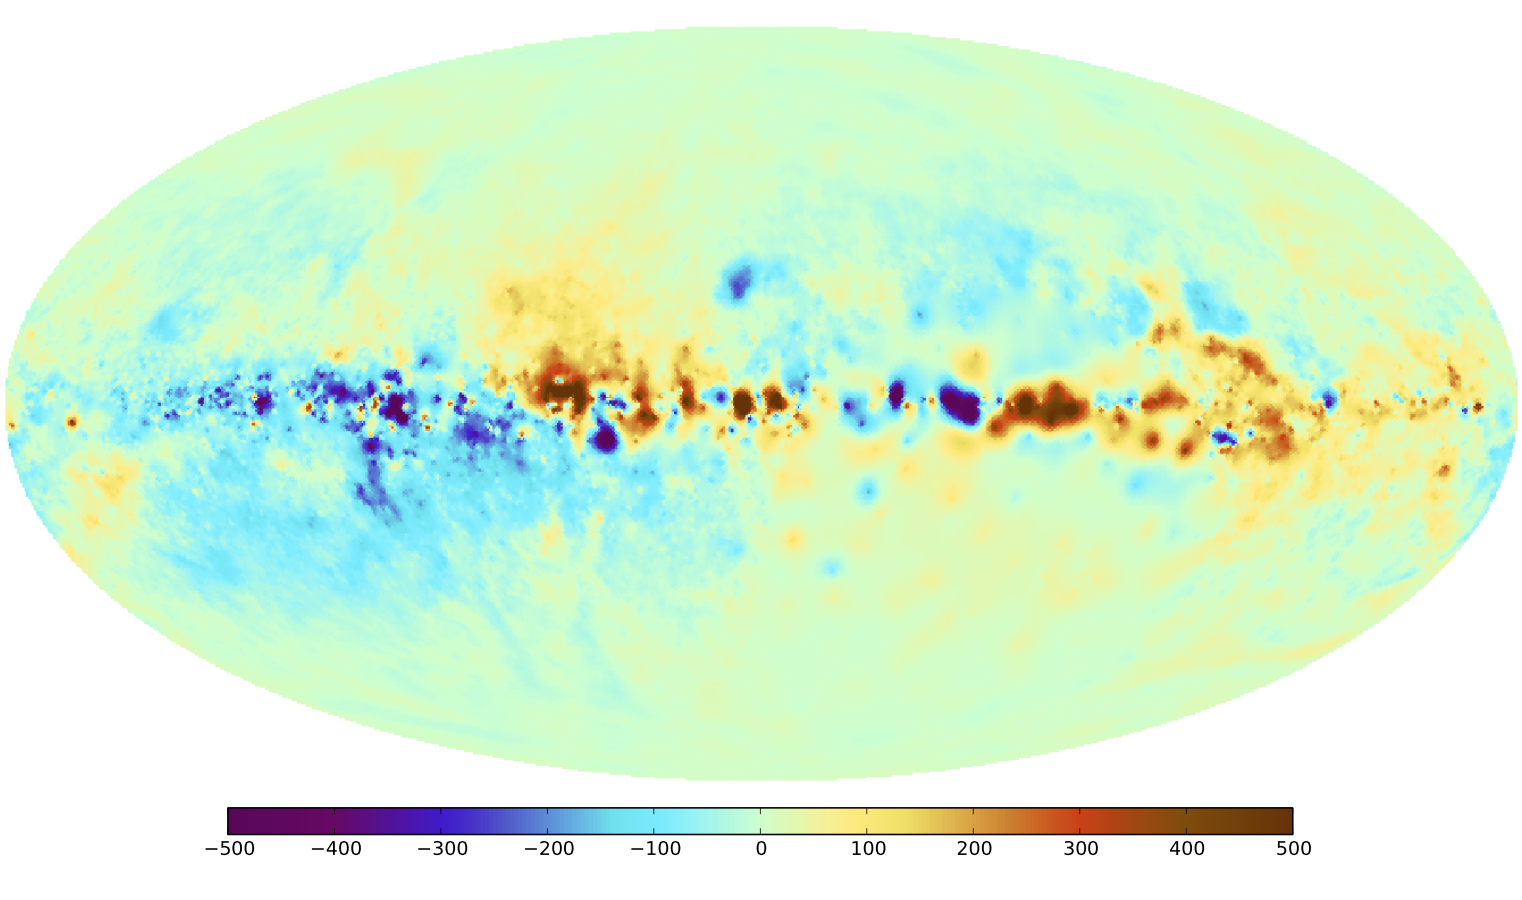
\includegraphics[width=0.7\textwidth]{chapters/astropol/figures/oppermann_map.png}
\caption[An all-sky map of RMs.]{An all-sky map of RMs. The colorbar has units of rad\,m$^{-2}$. Figure taken from \cite{Oppermann.12}.}
\label{fig:astropol_rm_map}
\end{figure}

\subsection{Depolarization}
\label{subsec:astropol_depolar}

Frequently the intrinsic polarization fraction of a radiating source much greater than the observed value; the observed radiation is `deopolarized'. Modes of depolarization can generally be categorized in to two groups: natural and instrumental. 

Instrumental polarization can occur via the beam -- the receptivity pattern, or point spread function (PSF) -- of the instrument (see Chapter~\ref{chapter:interferometry}). If the polarization angle changes significantly within the area of the beam, which is the case for turbulent Galactic magnetic fields and the very large beam areas of modern instruments (e.g. Chapter~\ref{chapter:instruments}), the observed polarization fraction can be attenuated during integration over the beam area. 
When probing RM distributions via RM synthesis, the channel width over which the data are averaged sets the sensitivity to the maximum RM by definition. Sources with higher RMs will suffer from `bandwidth depolarization', and this effect will strengthen at lower frequencies according to the phase-wrapping factor $2\Phi\lambda^2$.
As we explore in the next Chapter, interferometric polarization measurements are obtained by measuring the projection of the electric vector field on to orthogonal dipole arms. An electrical phase offset between the two arms will almost certainly exist in any instrument. If left uncalibrated, Stokes U will leak in to Stokes V, consequently depolarizing linear polarized intensity. Likewise, relatively faint polarized emission can be `washed-out' of measurements if Stokes I is able to leak in to Stokes Q and U measurements.

Natural depolarization can arise at the source of the radiation, due to turbulent magnetic fields. Different magnetic field projections along the line-of-sight can produce different angles of polarization, that can on average attenuate the observed polarized intensity. Similarly, radiation emitted from different depths of the source can undergo different amounts of Faraday rotation along the line-of-sight as they pass through regions of different electron densities. This effect is apparent in Figure~\ref{fig:astropol_drao_map}: in the plane of the Galaxy, which has a large column depth, the observed polarized intensity is low compared to, for example, the Northern Galactic Spur, which is physically closer to the Earth. 

Finally, the ionosphere of the Earth is a turbulent plasma, which when coupled with the Earth's magnetic field can act as a Faraday screen. If left uncorrected, averaging observations of the same patch of sky observed at different times can lead to a depolarization effect -- we explore this further in Chapter~\ref{chapter:ionosphere}.

As mentioned in Section~\ref{sec:astropol_linpol_fgs}, \cite{Bernardi.13} reported polarization fractions of extragalactic compact sources at 189\,MHz significantly lower than reported at higher frequencies. This was corroborated by some of the  measurements by \cite{Lenc.16}, although not all of the polarized point sources found in their survey showed significant evidence of depolarization. The least depolarized sources in that survey corresponded to hot-spots of large radio galaxies, which perhaps are not as deeply embedded in galactic plasma as the other sources observed, and therefore suffered less natural depolarization. \cite{Farnes.14} showed a systematic trend for depolarization of steep-spectrum point sources as frequency decreased, resulting in very low polarization fractions ($\ll 1\%$) below 300 MHz. They also suggested that natural polarization was the cause, due to turbulent magnetic fields at the source of the radiation.\\\\

Recall that in Chapter~\ref{chapter:eor_intro}, we stated that 21\,cm emission was effectively unpolarized. Why have we gone in to so much detail about polarized radiation? As we will see in subsequent Chapters, polarized power is capable of `leaking' in to Stokes I measurements through effects intrinsic to radiometric instruments, and calibration errors. Recall also that Faraday Rotation can induce spectral structure in otherwise smooth spectrum, polarized synchrotron emission. Coupled with leakage, this additional spectral structure risks contaminating the one lever-arm we have against the bright foregrounds! This effect lead to much of the research presented in this work.
